\documentclass{article}
\usepackage{graphicx}
\usepackage{caption}
\usepackage{subcaption}
\usepackage{float}

\begin{document}

\title{Estimating A Modified Ball-and-sticks Diffusion Model with Expectation Maximization and Rician Likelihood}
\author{Xinghua Zhu}

\maketitle

\begin{abstract}
  This is a summary of the modified ball-and sticks model estimation experiments.
\end{abstract}

%\section{Introduction}
%Here is the text of your introduction.


\section{Estimating weights V.S. diffusivities}
\subsection{Synthesized data}

\begin{enumerate}

\item{\textbf{Single compartment}}

DW signal is simulated with the multi-tensor model, with major and minor diffusivities ranging from $[1.3\times 10^{-3}, 2.1\times 10^{-3}]$ and $[2\times 10^{-4}, 5\times 10^{-4}]$, respectively. It is also assumed that the diffusivities in perpendicular directions are equal. When estimating the fiber compartment, the diffusivities are fixed at $(1.7e-3, 3e-4, 3e-4)$, while the weights are to be optimized. For each combination of diffusivities, the estimation is repeated for 200 times to test its stability.

Figure \ref{figOneFiber} are results of single compartment estimation. It is shown that the standard deviation of angular deviation and likelihood are very small, which indicates the algorithm converges stably over the 200 repetitions.

\begin{figure}[H]
  \caption{\label{figOneFiber}Single compartment estimation results}
  \begin{subfigure}{\textwidth}
    \centering
    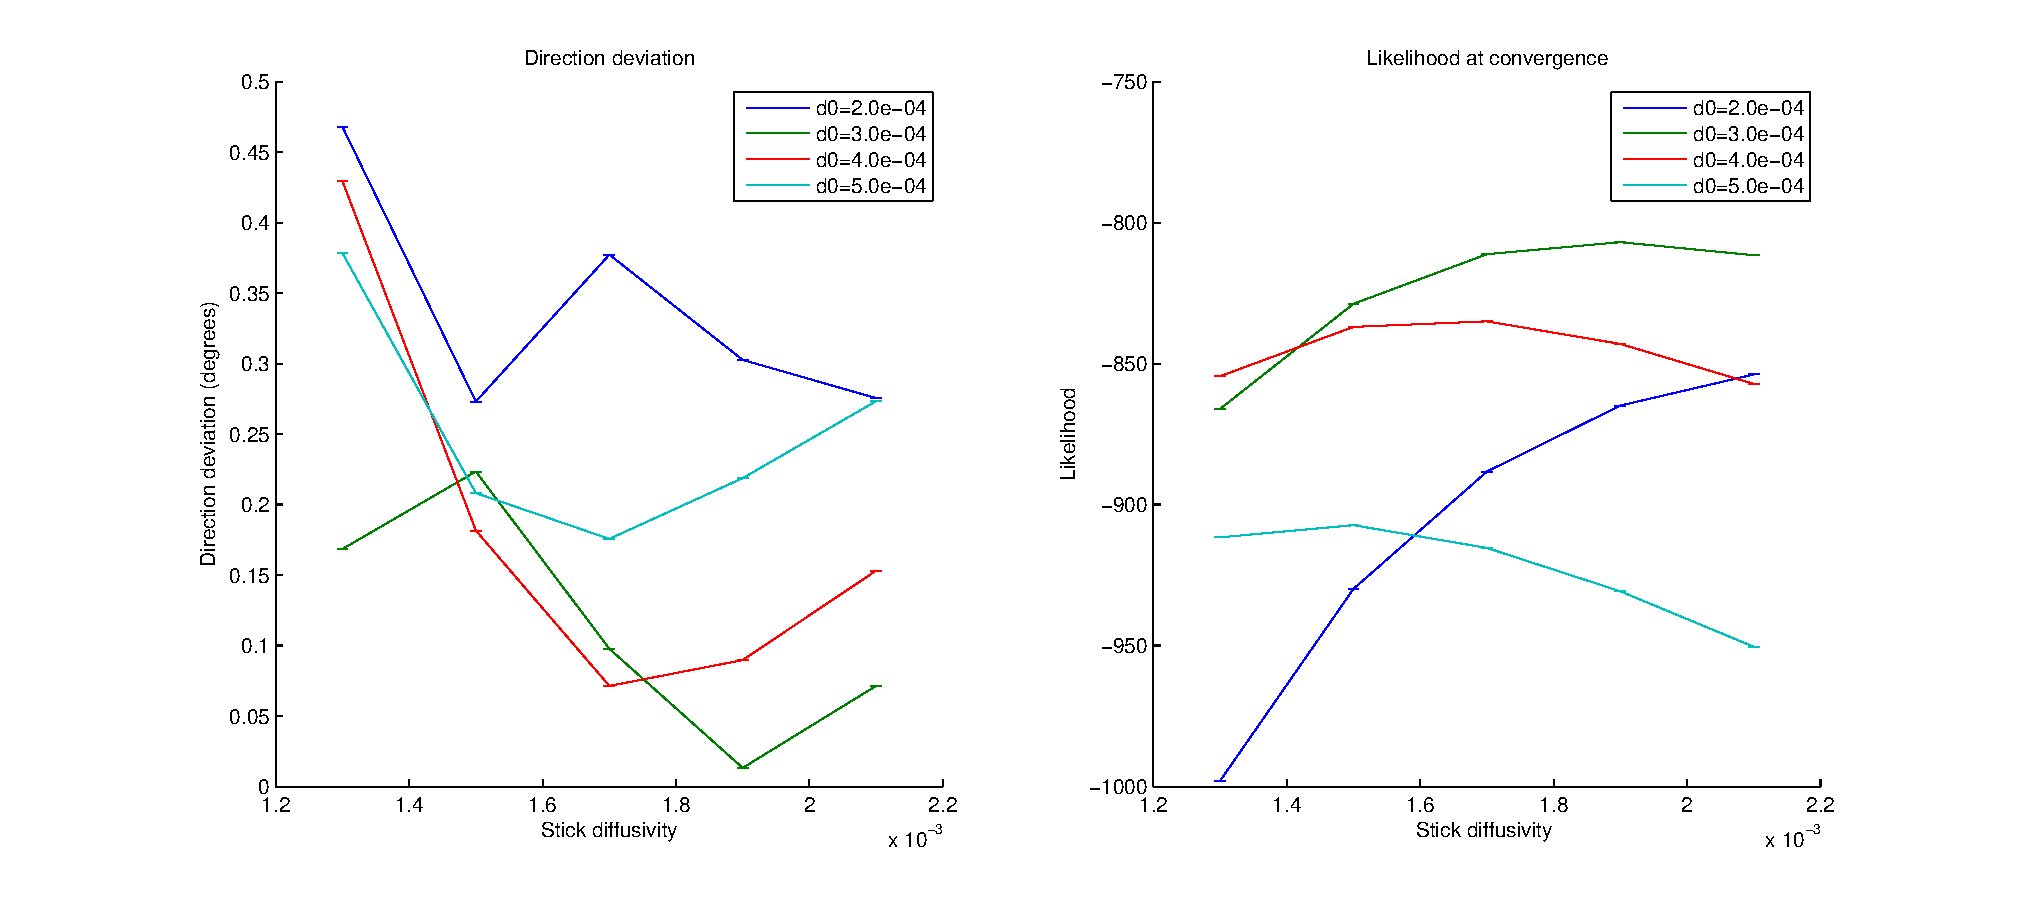
\includegraphics[width=\textwidth]{figures/one_fiber__snr=20.eps}
    \caption{SNR=20}
  \end{subfigure}
  \begin{subfigure}{\textwidth}
    \centering
    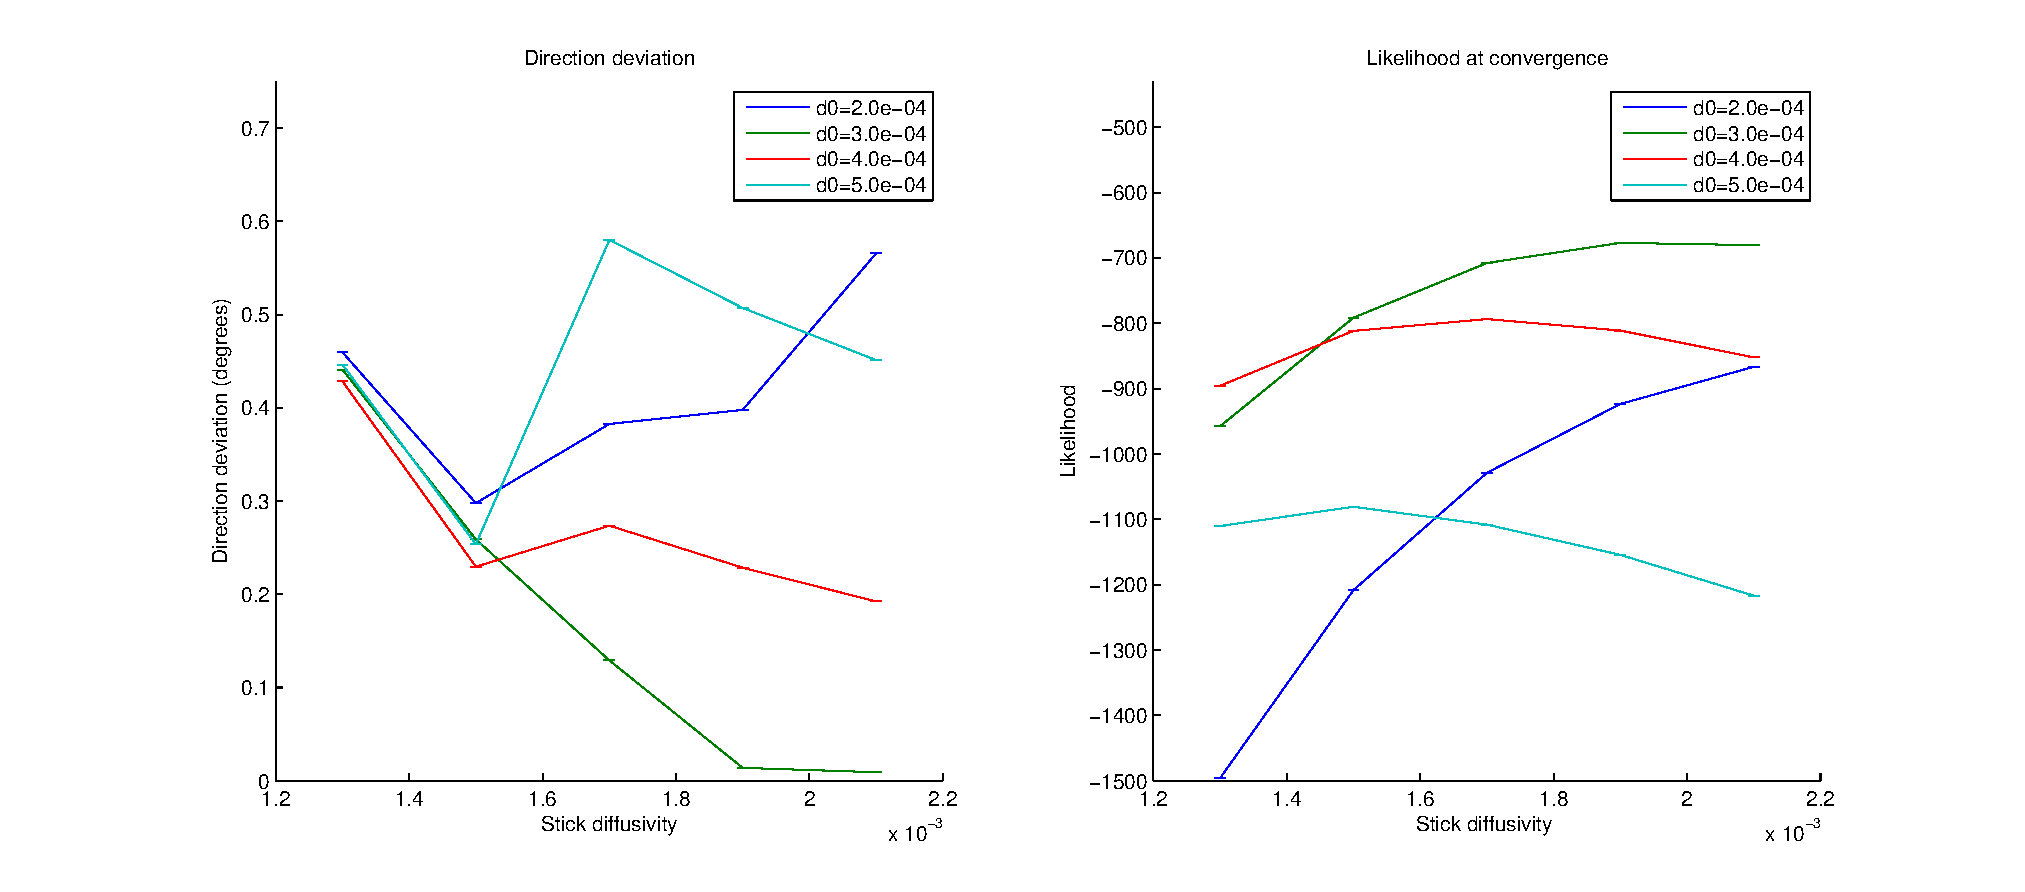
\includegraphics[width=\textwidth]{figures/one_fiber__snr=40.eps}
    \caption{SNR=40}
  \end{subfigure}
\end{figure}

\item \textbf{Two compartments}

In the simulation of two-compartment DW signals, each compartment is simulated the same way as single multi-tensor compartment. Figure \ref{figTwoFibers1} and \ref{figTwoFibers2} are results of two-compartment estimation. Solid lines stand for mean and standard deviation of the mean angular deviation between the two compartments, while the dashed ones stand for the maximum deviation between the two compartments.

\begin{figure}[H]
  %\begin{subfigure}{\textwidth}
    \centering
    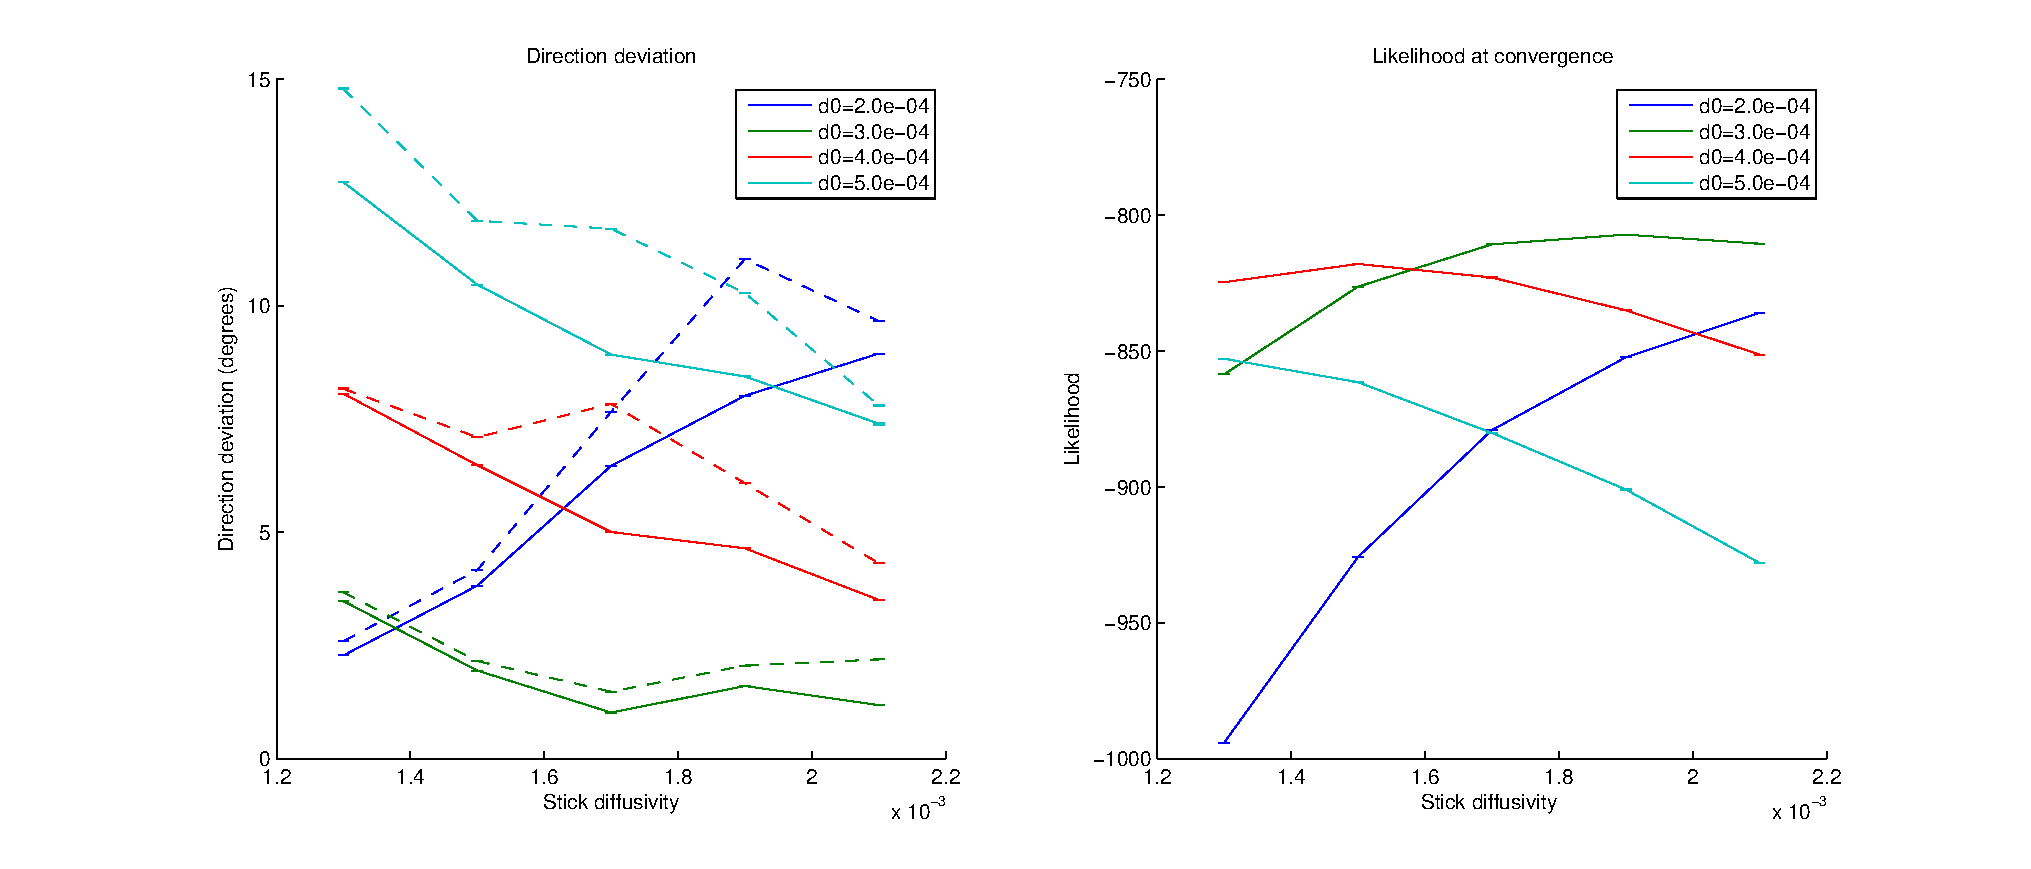
\includegraphics[width=\textwidth]{figures/two_fiber__snr=20__angle=30.eps}
    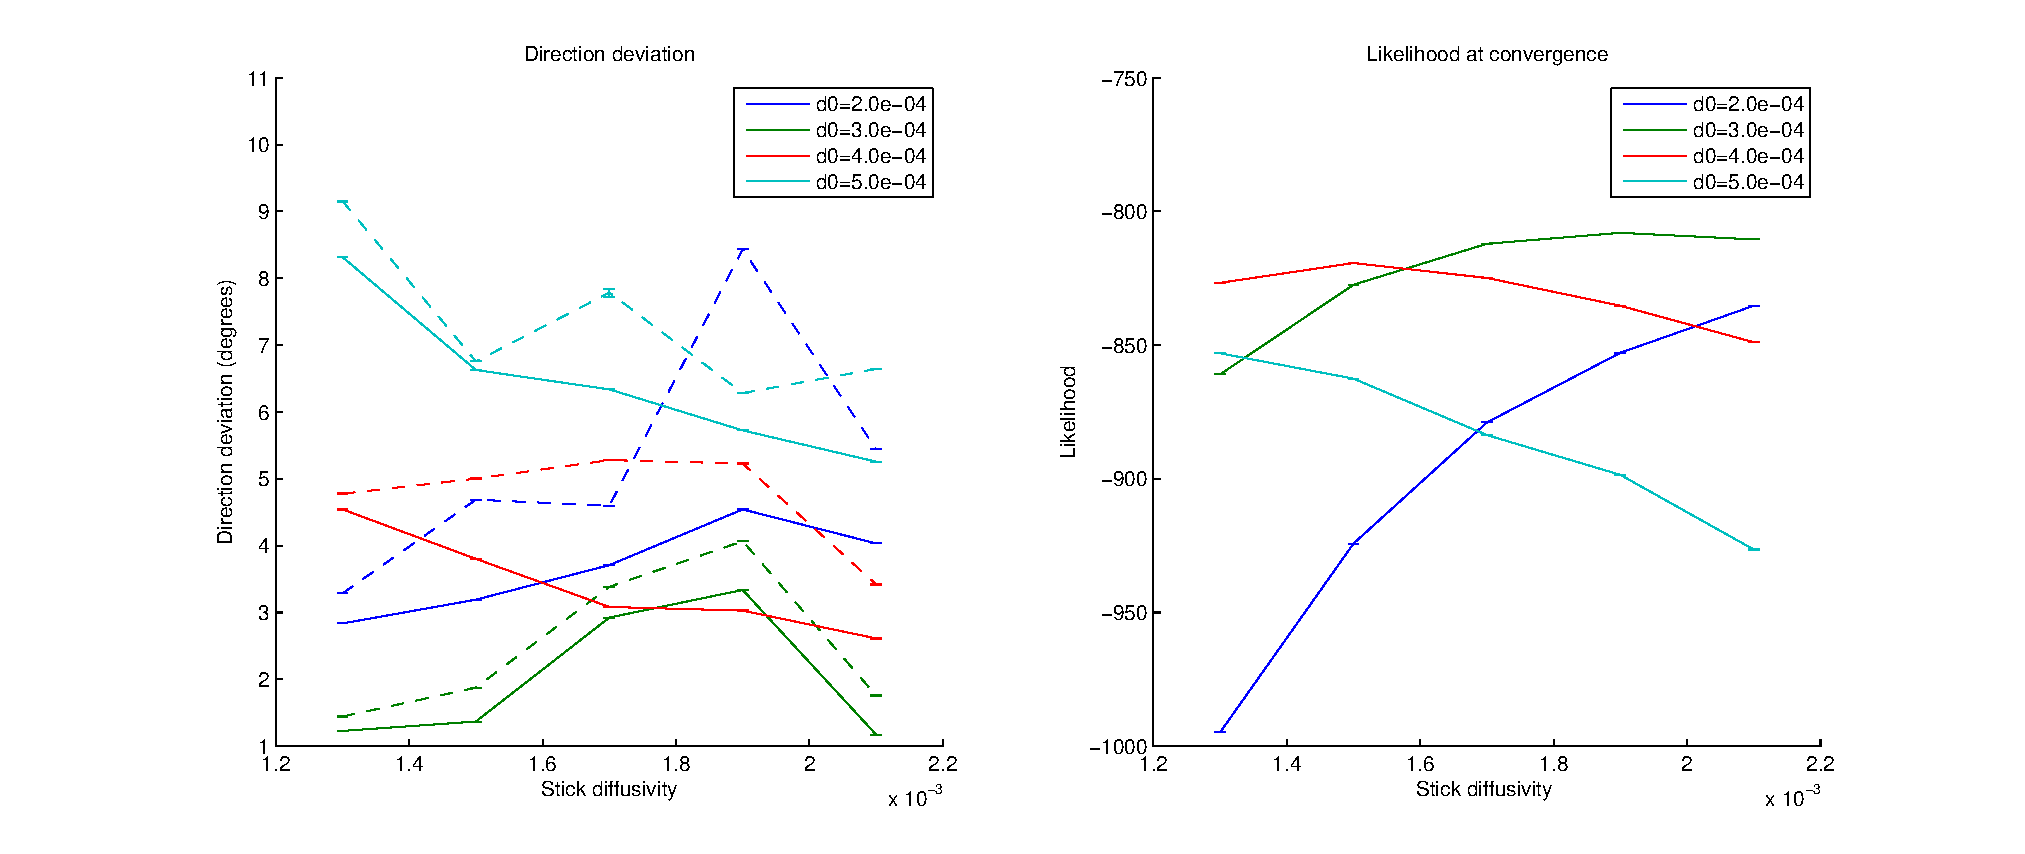
\includegraphics[width=\textwidth]{figures/two_fiber__snr=20__angle=45.eps}
    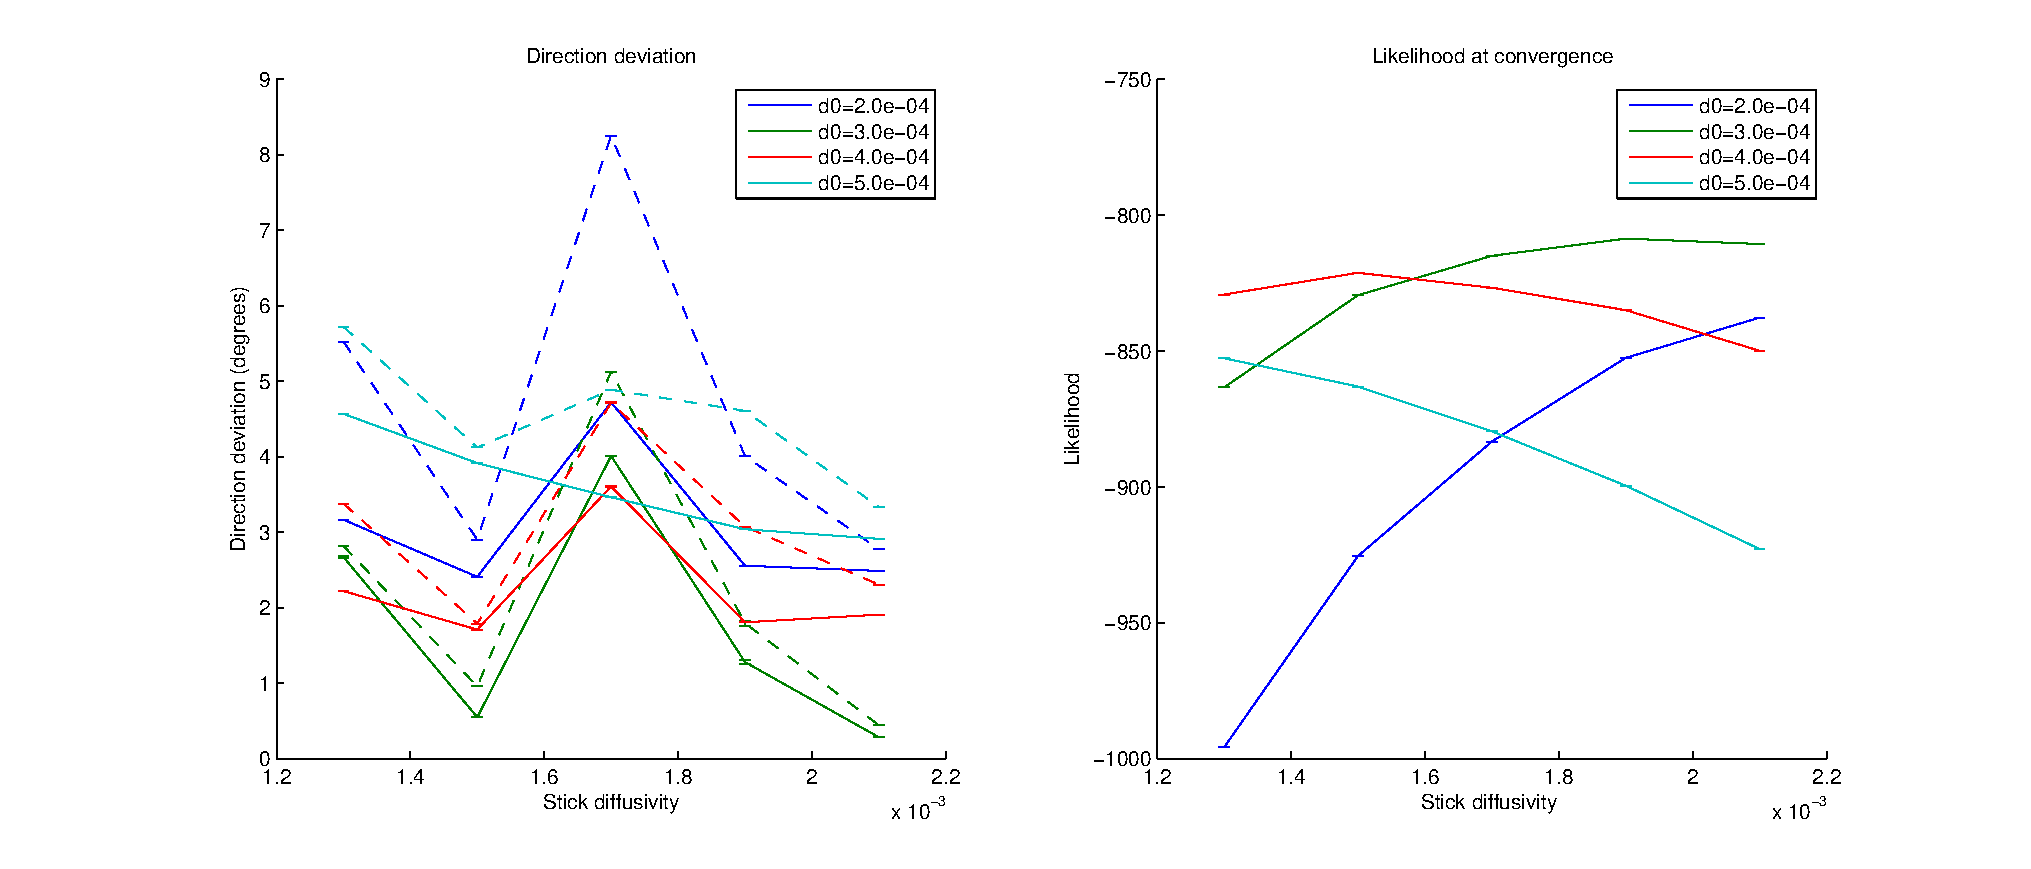
\includegraphics[width=\textwidth]{figures/two_fiber__snr=20__angle=60.eps}
    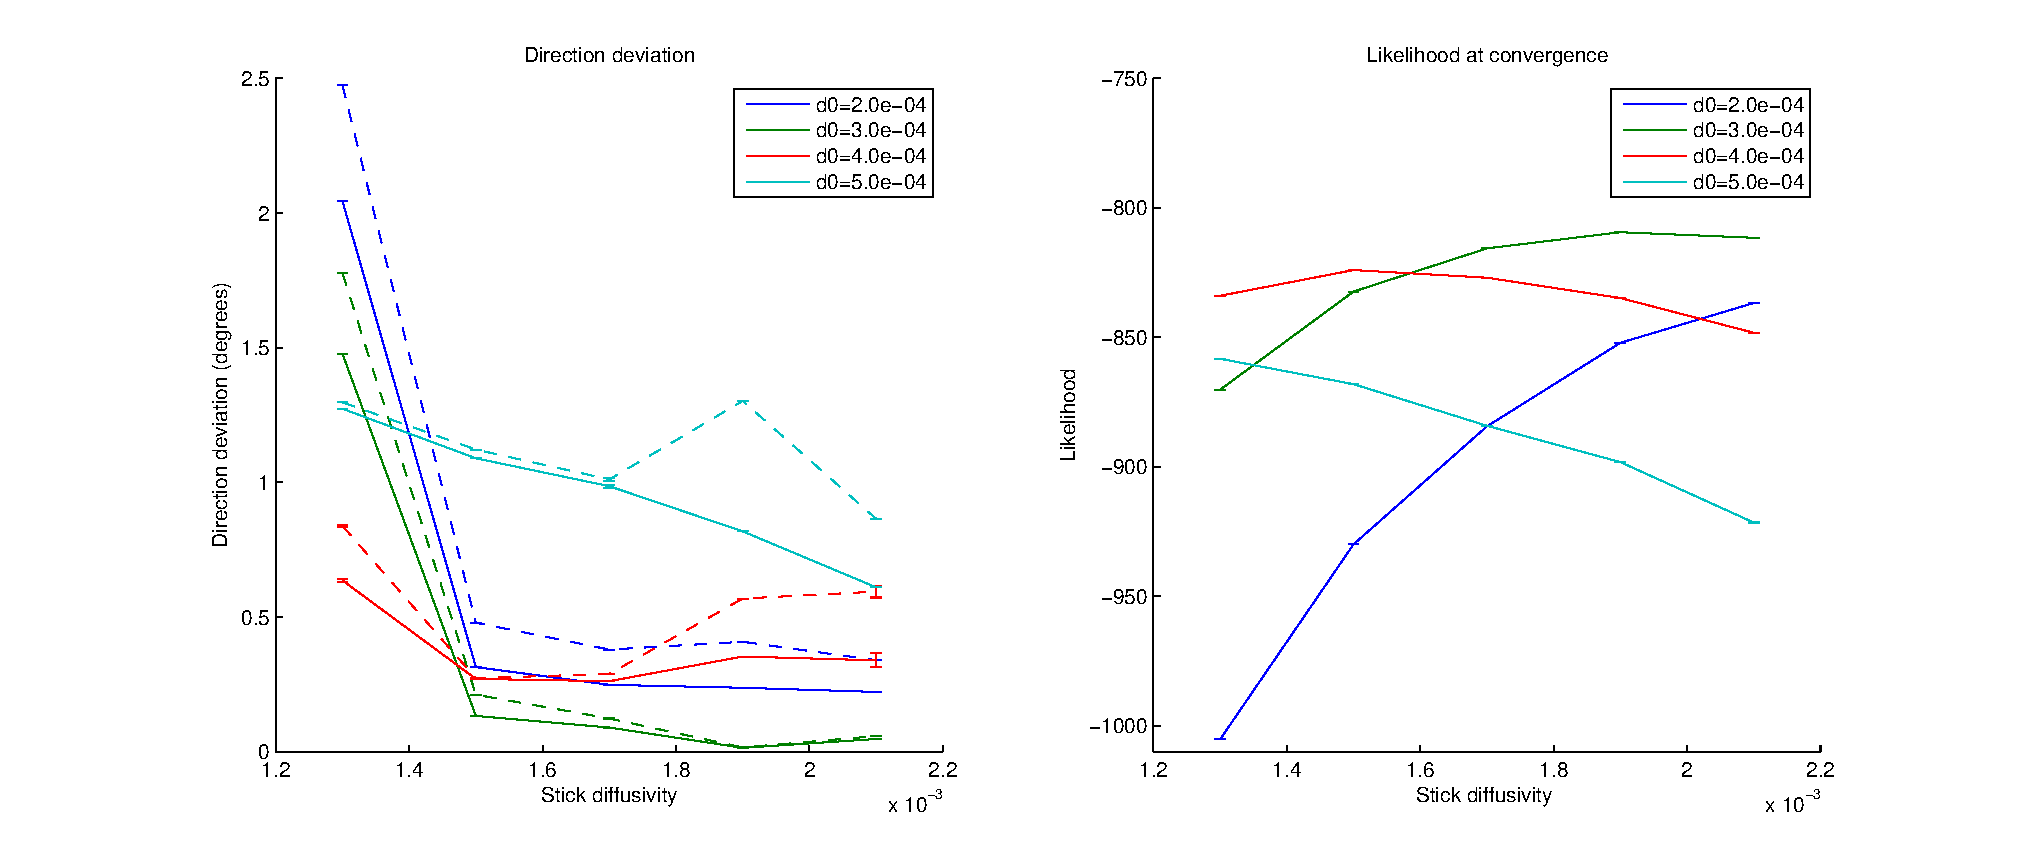
\includegraphics[width=\textwidth]{figures/two_fiber__snr=20__angle=90.eps}
    \caption{\label{figTwoFibers1}Two compartment estimation results: SNR=20. From top to bottom: separation angle 30, 45, 60 and 90 degrees}
  %\end{subfigure}
\end{figure}
  
\begin{figure}[H]
  %\begin{subfigure}{\textwidth}
    \centering
    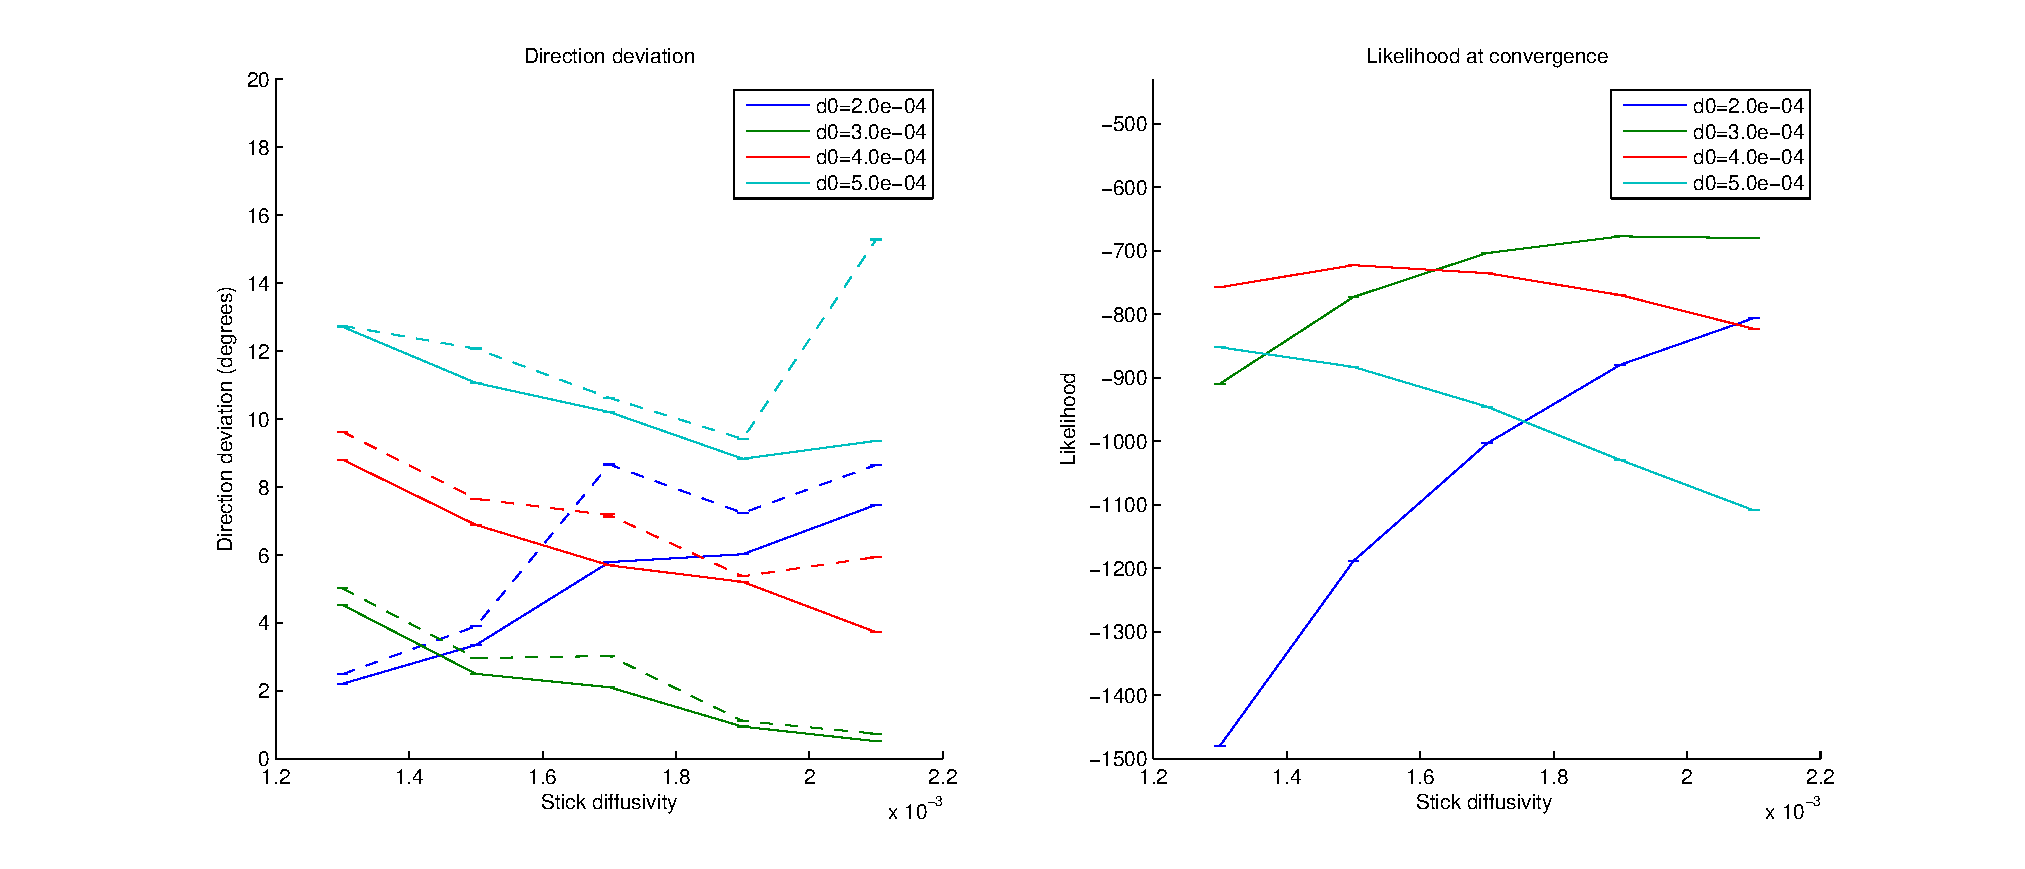
\includegraphics[width=\textwidth]{figures/two_fiber__snr=40__angle=30.eps}
    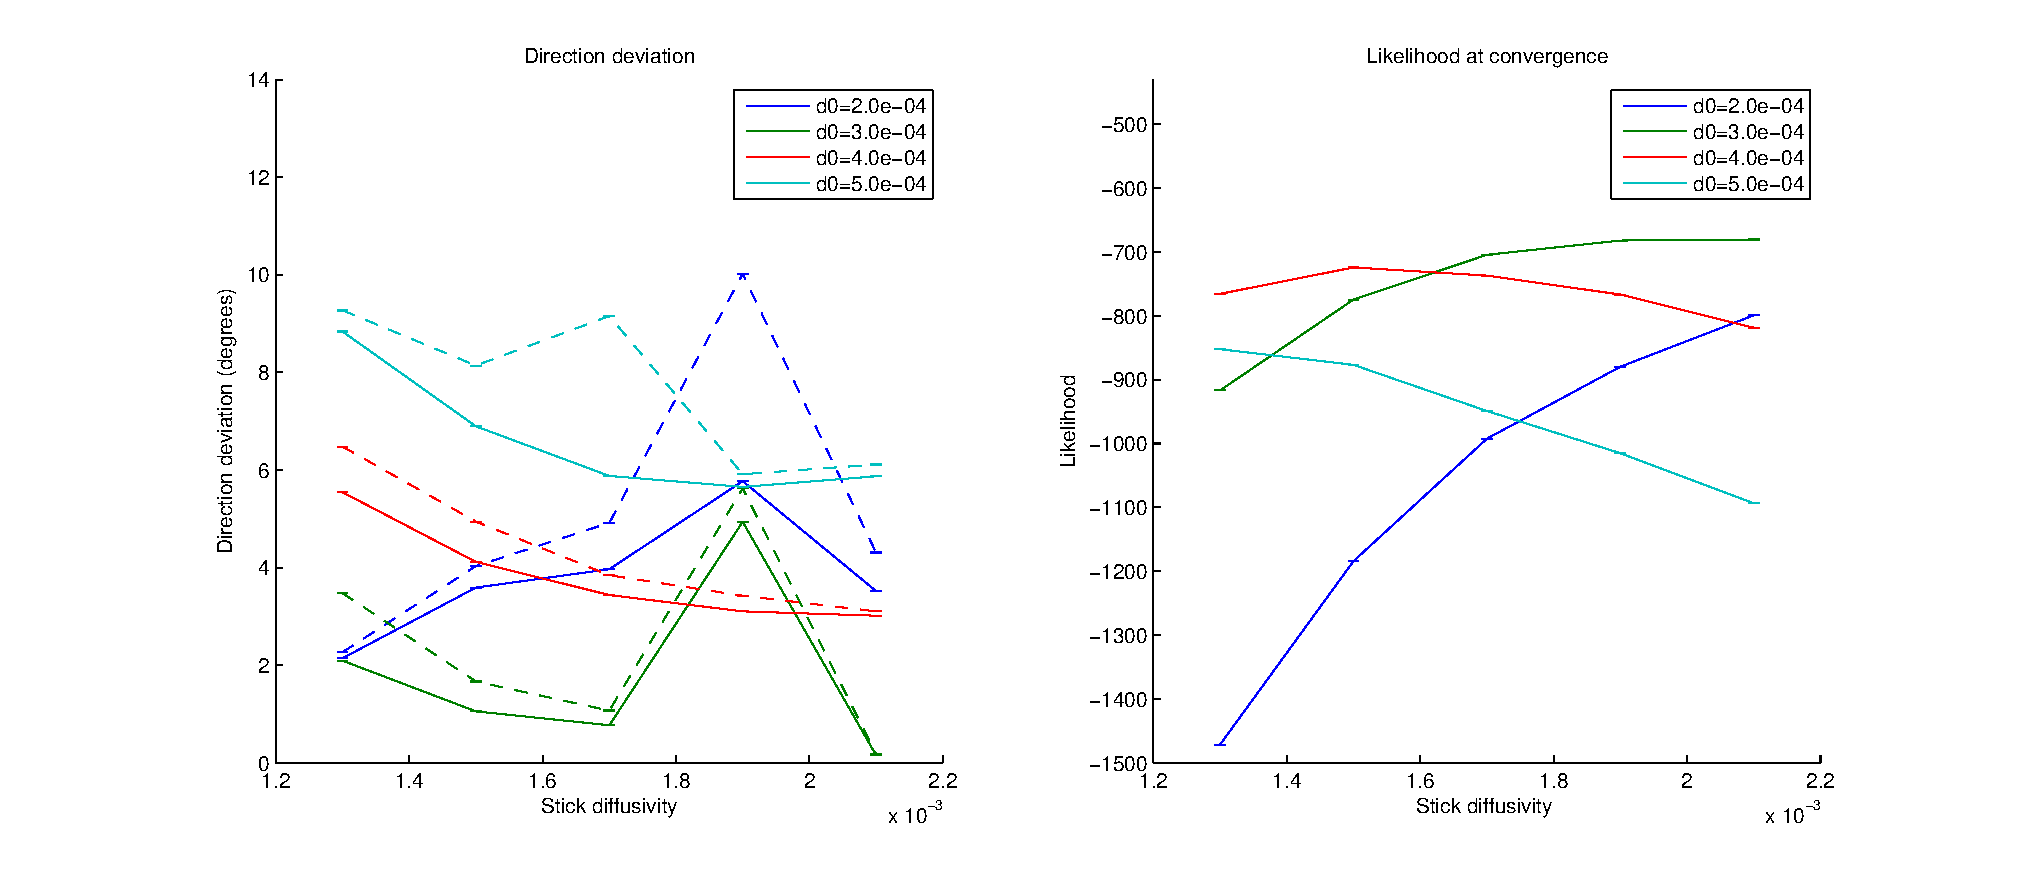
\includegraphics[width=\textwidth]{figures/two_fiber__snr=40__angle=45.eps}
    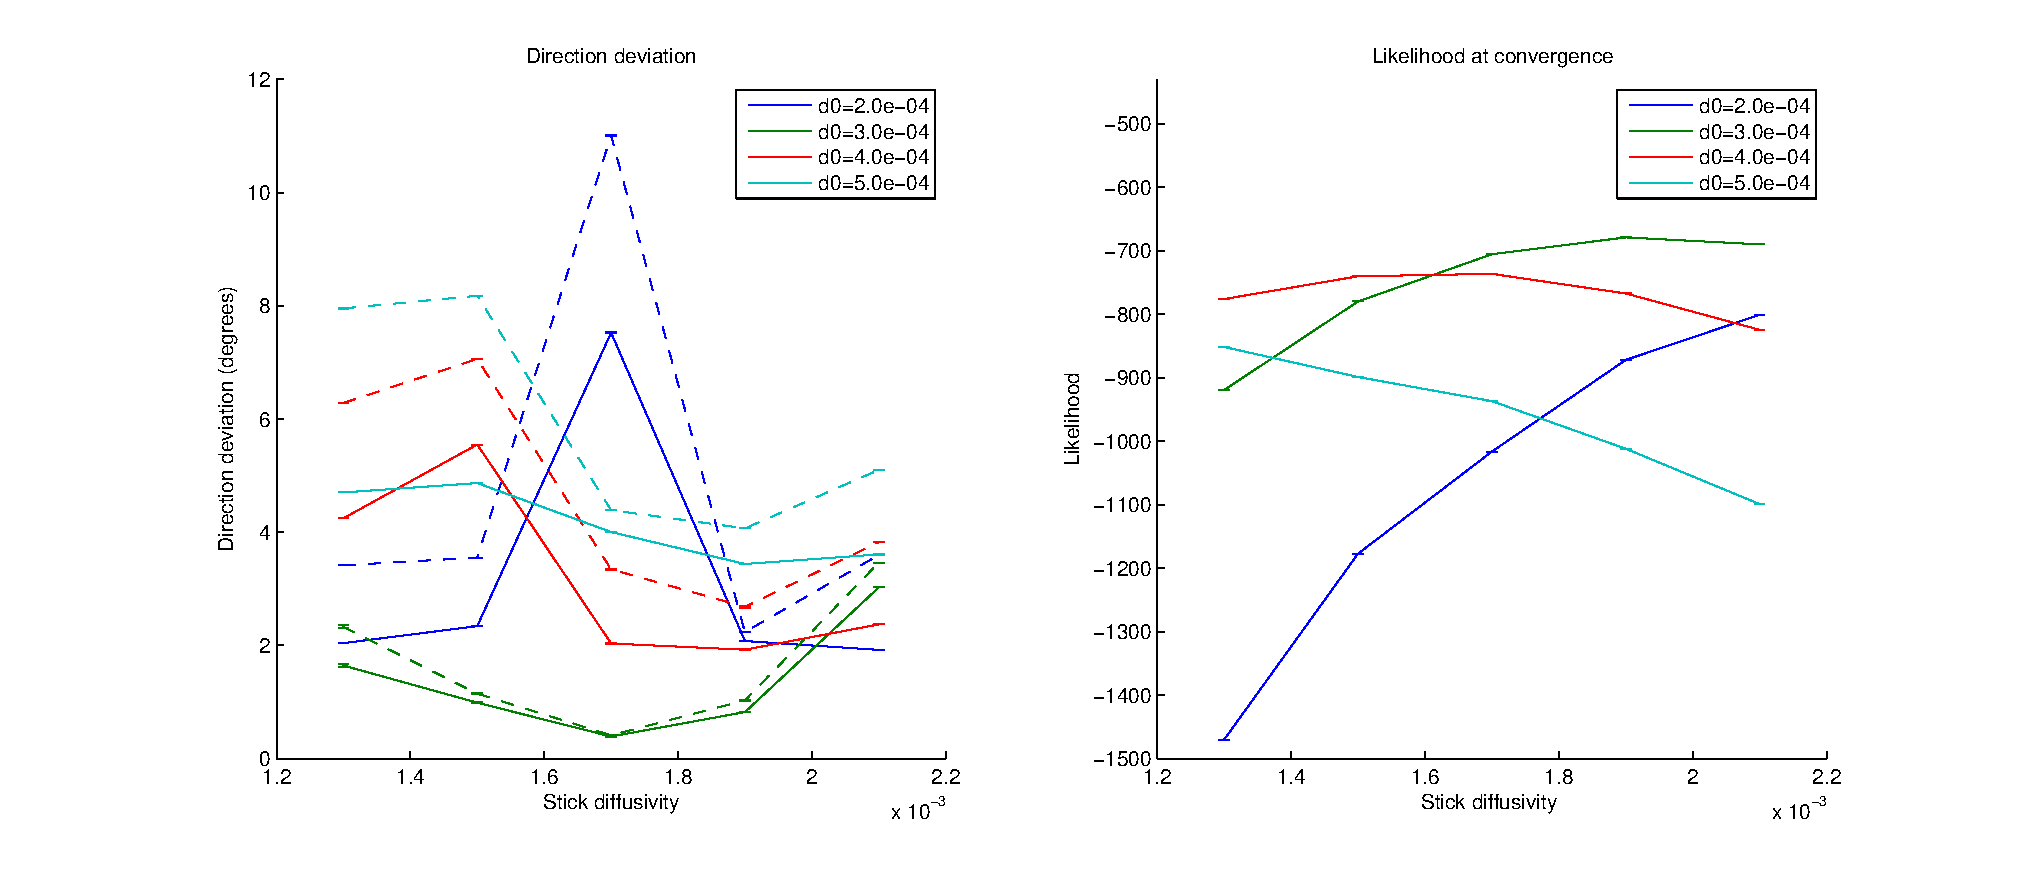
\includegraphics[width=\textwidth]{figures/two_fiber__snr=40__angle=60.eps}
    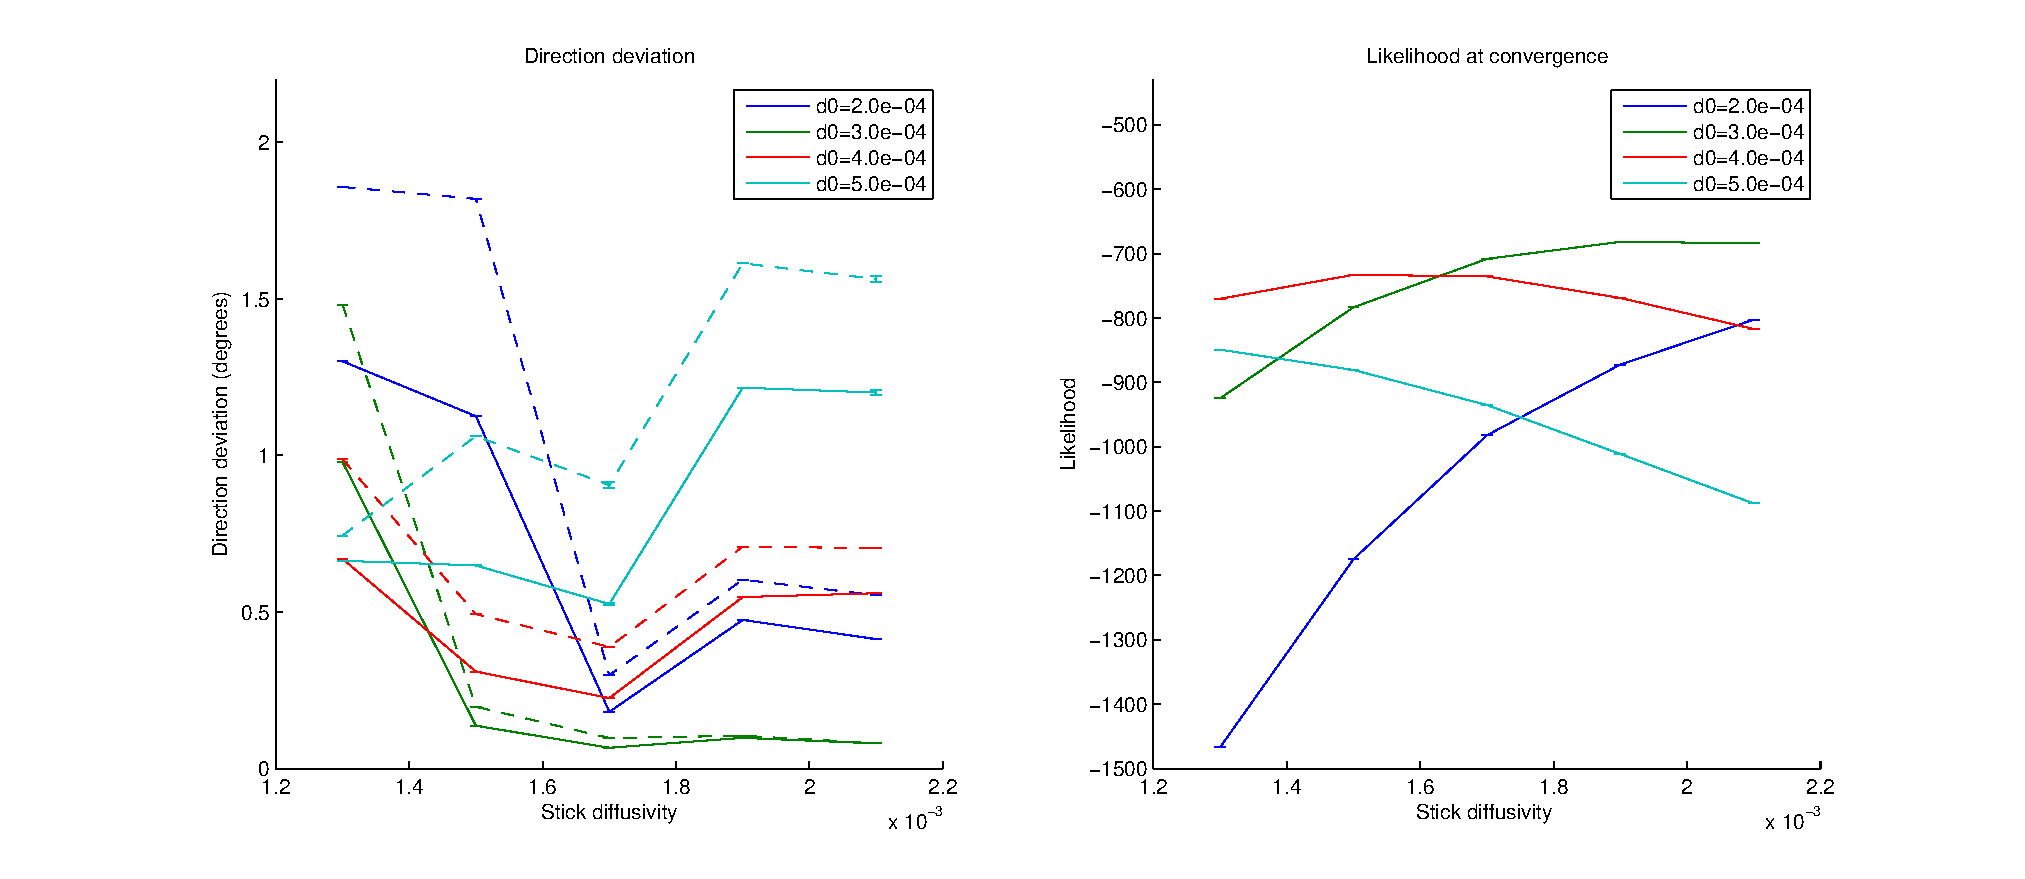
\includegraphics[width=\textwidth]{figures/two_fiber__snr=40__angle=90.eps}
    \caption{\label{figTwoFibers2}Two compartment estimation results: SNR=40. From top to bottom: separation angle 30, 45, 60 and 90 degrees}
  %\end{subfigure}
\end{figure}


\end{enumerate}

\subsection{Phantom data}

\begin{enumerate}
  \item Estimating diffusivities with fixed equal weights. Figure \ref{figPhantomDiffus}.

    \begin{figure}[H]
      \caption{\label{figPhantomDiffus}Estimation results of MICCAI phantom data with diffusivity estimation}
      \centering
      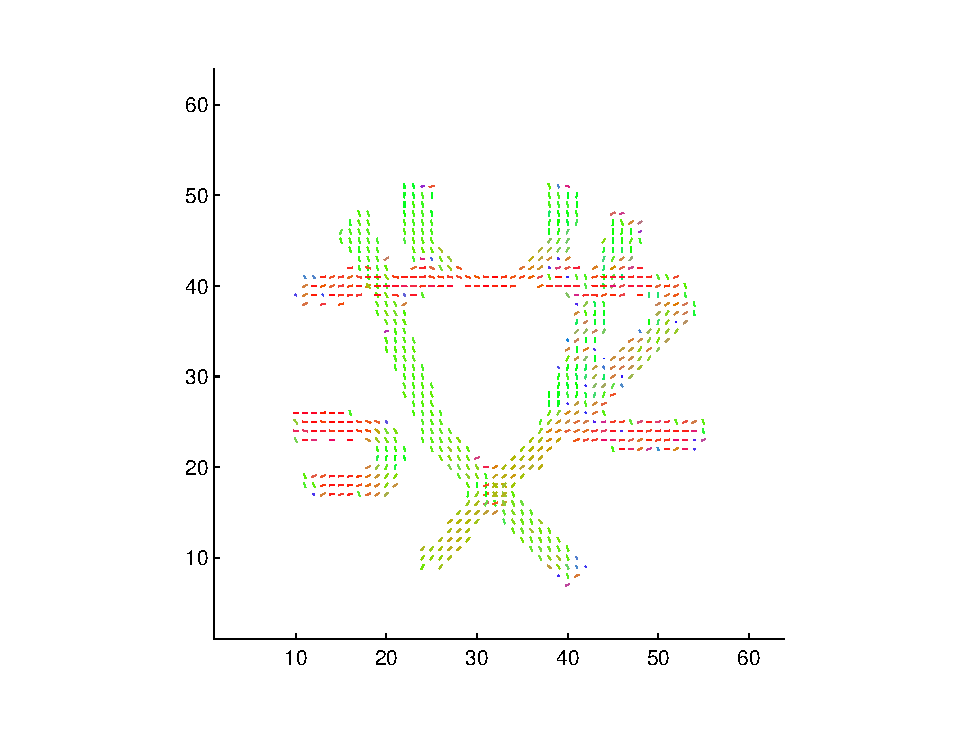
\includegraphics[width=0.8\textwidth]{figures/phantom_diffus.eps}
      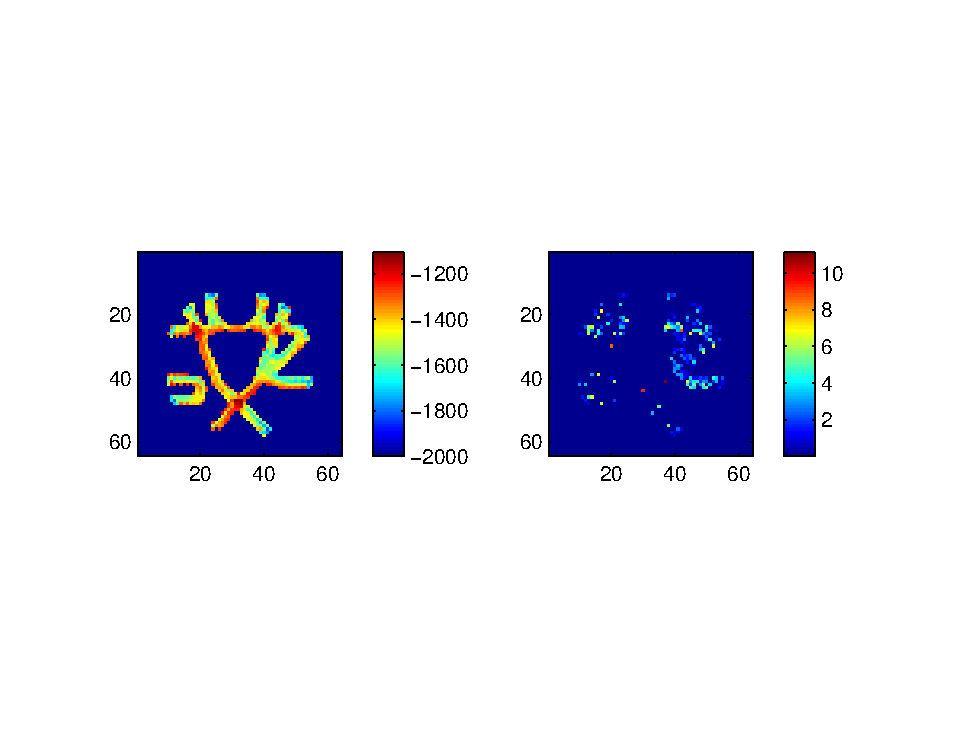
\includegraphics[width=\textwidth]{figures/phantom_diffus_like.eps}
    \end{figure}

  \item Estimating weights with diffusivities fixed at $(2.5\times 10^{-3}, 1.2\times 10^{-3}, 1.2\times 10^{-3})$. Figure \ref{figPhantomWeights}.

    \begin{figure}[H]
      \caption{\label{figPhantomWeights}Estimation results of MICCAI phantom data with weight estimation}
      \centering
      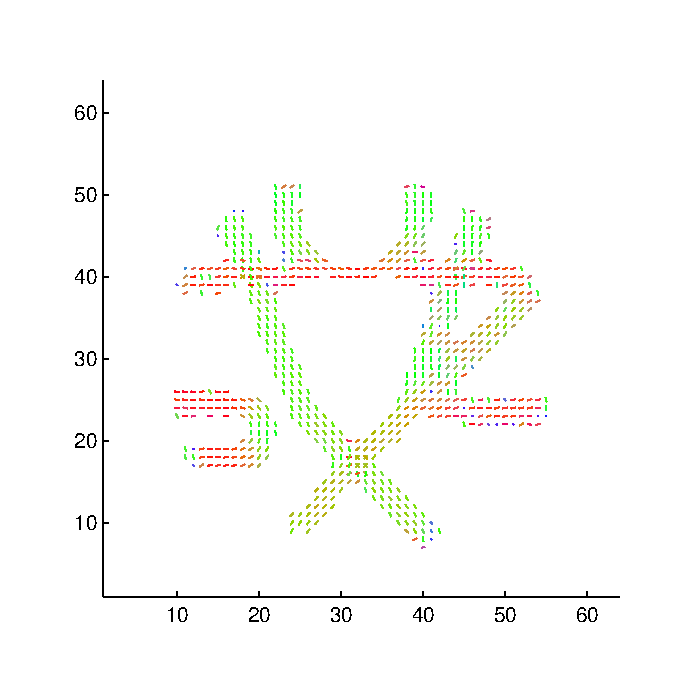
\includegraphics[width=0.8\textwidth]{figures/phantom_weights.eps}
      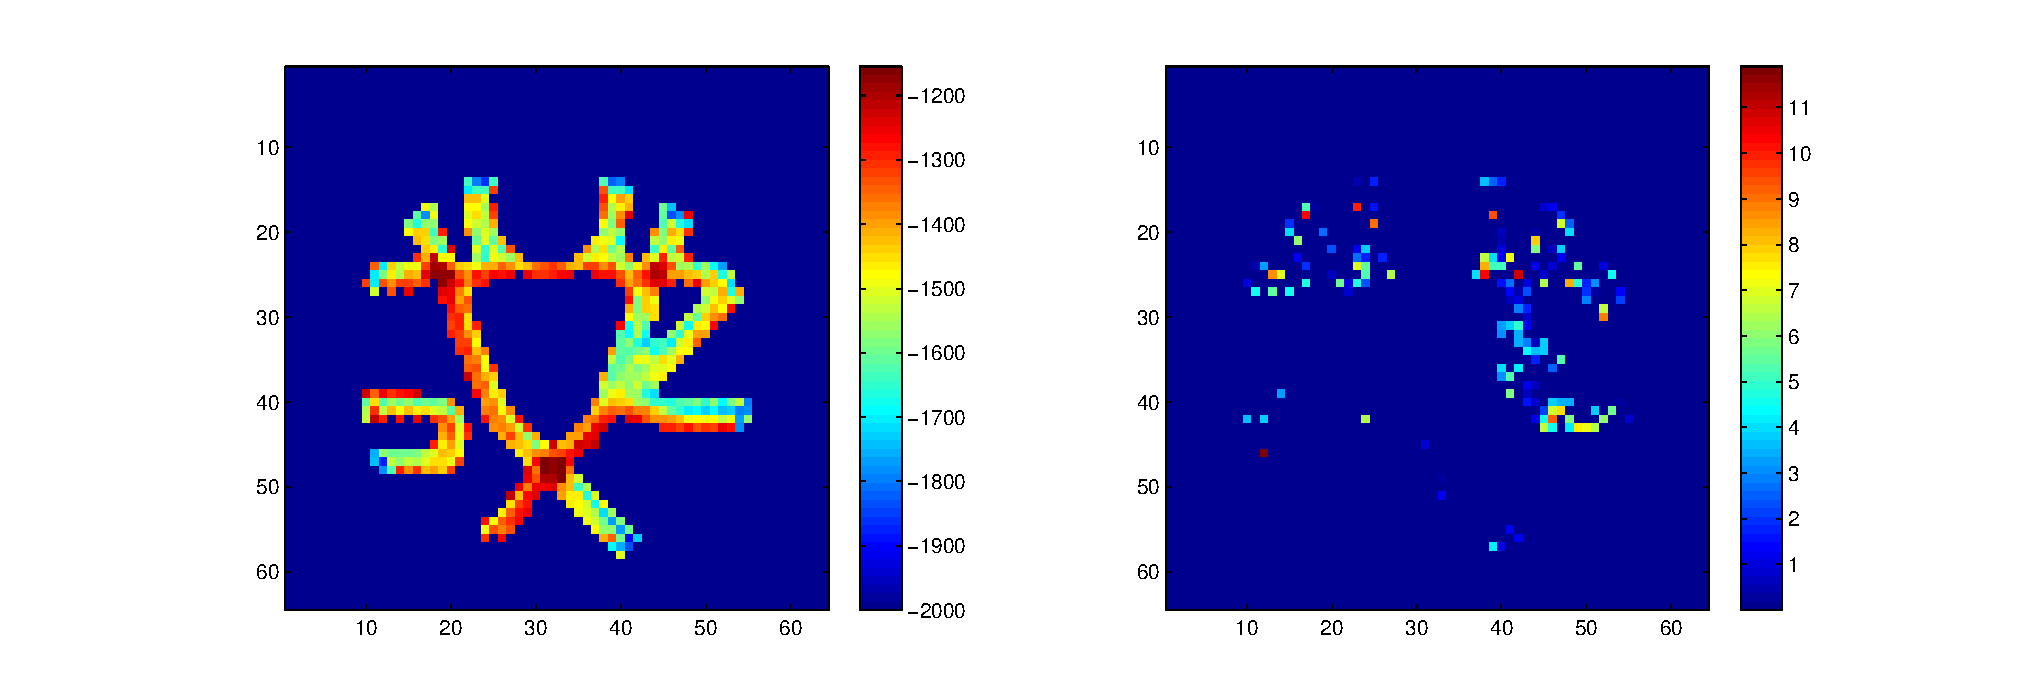
\includegraphics[width=\textwidth]{figures/phantom_weights_like.eps}
    \end{figure}
\end{enumerate}

%\section{Conclusion}
%Write your conclusion here.

\end{document}